\documentclass[a4paper]{article}
\usepackage[utf8]{inputenc}
\usepackage[spanish, es-tabla, es-noshorthands]{babel}
\usepackage[table,xcdraw]{xcolor}
\usepackage[a4paper, footnotesep = 1cm, width=20cm, top=2.5cm, height=25cm, textwidth=18cm, textheight=25cm]{geometry}
%\geometry{showframe}

\usepackage{tikz}
\usepackage{amsmath}
\usepackage{amsfonts}
\usepackage{amssymb}
\usepackage{float}
\usepackage{graphicx}
\usepackage{caption}
\usepackage{subcaption}
\usepackage{multicol}
\usepackage{multirow}
\setlength{\doublerulesep}{\arrayrulewidth}
\usepackage{booktabs}

\usepackage{hyperref}
\hypersetup{
    colorlinks=true,
    linkcolor=blue,
    filecolor=magenta,      
    urlcolor=blue,
    citecolor=blue,    
}

\newcommand{\quotes}[1]{``#1''}
\usepackage{array}
\newcolumntype{C}[1]{>{\centering\let\newline\\\arraybackslash\hspace{0pt}}m{#1}}
\usepackage[american]{circuitikz}
\usetikzlibrary{calc}
\usepackage{fancyhdr}
\usepackage{units} 

\graphicspath{{../Calculos-Potencia/}{../Caracteristicas/}{../Consideraciones/}{../Gain-Stage/}{../Input-Stage/}{../Output-Stage/}{../Simulaciones/}{../Alimentacion/}{../Conclusiones/}}

\pagestyle{fancy}
\fancyhf{}
\lhead{22.12 Electrónica II}
\rhead{Mechoulam, Lambertucci, Rodriguez, Londero, Scala}
\rfoot{Página \thepage}

\begin{document}

\tableofcontents
\newpage
%%%%%%%%%%%%%%%%%%%%%%%%%%%%%%%%%%%%%%%%%%%%%%%%%%%%%%%%%%%%%%%%%%%%%%
\subsection{Diseño Propuesto}

En la siguiente instancia se realiza una fuente de tensión regulada, la cual se ajusta a las especificaciones de:
\begin{align}
0V \leq V_o \leq 9V \ \ \ \ \ \ \wedge \ \ \ \ \ \ I_{o-Max}=2.5A
\end{align}

Se optó por un diseño que muestre tensión y sume corriente, siendo el diseño elegido para la fuente el presentado a continuación.
\begin{figure}[H]
\centering
	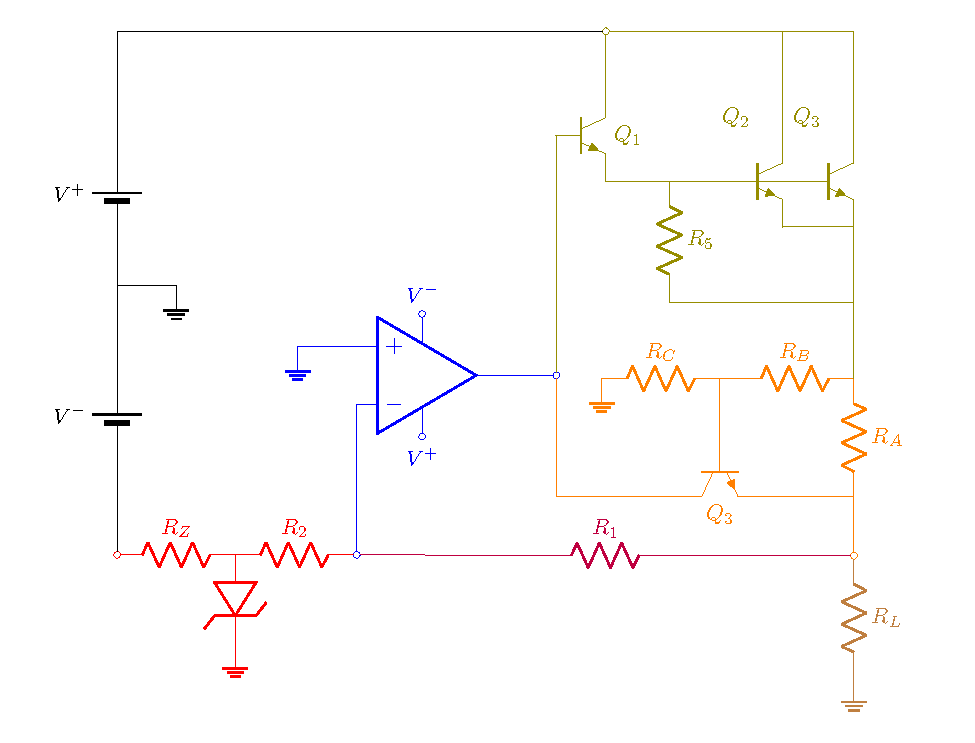
\includegraphics[width=0.8\textwidth, page=1]{ImagenesEjercicio2/Regulador.pdf}
	\caption{Circuito regulador de tensión propuesto.}
	\label{fig:circuitoprop}
\end{figure}

Dicho circuito puede ser separado en 5 bloques fundamentales:
\begin{itemize}
\item \textcolor{blue}{Amplificador error}
\item \textcolor{olive}{Transistor de paso}
\item \textcolor{red}{Elemento de referencia}
\item \textcolor{purple}{Circuito de detección}
\item \textcolor{orange}{Circuito de protección}
\end{itemize}

 


\subsubsection{Análisis de realimentación negativa}
\label{sec:realimentacion-negativa}

La teoría de la realimentación negativa plantea que dado un sistema a lazo cerrado ideal, con un número impar de inversiones de fase, la ganancia de este puede aproximarse como la inversa del factor de realimentación si la ganancia de lazo en módulo es mucho mayor a la unidad, es decir
\begin{equation}
P.E. = \frac{A }{1+ f \cdot A} = \frac{1}{f} \cdot \frac{|T|}{1 + |T|}
\end{equation}
donde $A$ es la respuesta a lazo abierto, $f$ el factor de realimentación y $T$ es la ganancia de lazo. Se puede observar que bajo las condiciones descritas anteriormente, se tiene entonces que 

\begin{equation}
P.E. \approx \frac{1}{f}
\end{equation}

\begin{figure}[H]
\centering
	\includegraphics[width=0.8\textwidth, page=4]{ImagenesEjercicio2/Regulador.pdf}
	\caption{Lazo de realimentación negativa.}
	\label{fig:circuito_lazo}
\end{figure}

En el circuito realizado puede observarse un lazo de realimentación negativa el cual posee una inversión de fase producida por el amplificador operacional detallado en la Figura (\ref{fig:circuito_lazo}). También es de interés observar los siguientes puntos: 
\begin{itemize}
\item Por tierra virtual, el opamp trabaja para mantener la tensión nula en su terminal negativo.
\item El diodo zener consume la corriente necesaria para mantener la caída de tensión sobre este fija.
\item El lazo de realimentación trata de fijar una tensión a la salida de la fuente regulada.
\end{itemize}

Teniendo en cuenta dichos aspectos, es de notar que la fuente realiza un muestreo de tensión a la salida mediante la resistencia $R_1$, la cual inyecta una corriente proporcional a la dicha, realizándose una suma de corrientes en el nodo del terminal negativo del amplificador operacional, siendo la referencia la corriente fija proporcionada por la resistencia $R_2$.

En resumidas cuentas, el parámetro estabilizado del sistema es

\begin{equation}
P.E. = \frac{V_o}{I_N} = -\frac{V_o \cdot R_2}{|V_z|} = \frac{1}{f} \cdot \frac{|T|}{1 + |T|}
\end{equation}

Luego, se puede demostrar que la ganancia $f$ se puede aproximar como la razón entre el parámetro que se suma en el lazo y el parámetro que se muestrea, cuando la tensión en el nodo del terminal negativo del opamp es cero, obteniendo así
\begin{equation}
f \approx -\frac{1}{R_1}
\end{equation}

Si se considera que la ganancia de lazo en módulo es mucho mayor que la unidad dado que se utiliza un opamp como amplificador, se obtiene finalmente que
\begin{equation}
V_o = |V_z| \cdot \frac{R_1}{R_2}
\label{eq:vovz}
\end{equation}

\subsection{Bloques del Regulador}
\subsubsection{Elemento de Referencia}

El elemento de referencia (o también llamado entrada o generador en un circuito de realimentación negativa) proporciona la tensión de entrada al sistema, la cual comparte nodo con el amplificador error y el circuito de detección, como se mencionó anteriormente.

En cuanto al funcionamiento, el zener está polarizado por $V^{-}$ y $R_Z$. Esta etapa del sistema s prácticamente independiente del resto del circuito, y además debe ser altamente estable, es por ello que se utiliza $R_Z >> r_Z$ para evitar variaciones de $V_Z$, es decir, de la tensión de referencia, con respecto a $V^{-}$. Para ello se plantea las ecuaciones propias del nodo $V_Z$: 
\begin{figure}[H]
\centering
	\includegraphics[width=0.5\textwidth, page=6]{ImagenesEjercicio2/Regulador.pdf}
	\caption{Circuito de transistor de paso.}
	\label{fig:transistorDePaso}
\end{figure}

\begin{equation*}
	\frac{V^{-} - V_Z}{R_Z} + I_Z = \frac{V_Z - V_1}{R_2} \approx \frac{V_Z}{R_2}
\end{equation*}
\begin{equation*}
	V^{-} - V_Z = \left( \frac{V_Z}{R_2} - I_Z \right) \cdot \frac{1}{R_Z}
\end{equation*}
\begin{equation}
	R_Z = R_2 \cdot \frac{V^{-} - V_Z}{V_Z - R_2 I_Z}
	\label{eq:referencia}
\end{equation}

\subsubsection{Circuito de Detección}
\label{sec:circuito-de-deteccion}

El circuito de detección está compuesto por la resistencia $R_2$. La caída de potencial sobre esta depende solamente de la tensión a la salida de la fuente, lo que permite generar una corriente proporcional a esta.

\begin{figure}[H]
\centering
	\includegraphics[width=0.5\textwidth, page=7]{ImagenesEjercicio2/Regulador.pdf}
	\caption{Circuito de detección.}
	\label{fig:circdeteccion}
\end{figure}

 De esta manera, se genera una resta de corrientes en el nodo del terminal negativo del operacional, siendo estas la corriente suministrada por la $R_2$, la corriente fija suministrada por la $R_1$, y la corriente del terminal negativo del opamp. Denominaremos a esta última corriente como el error de la fuente regulada.

\subsubsection{Amplificador de Error y Pre-regulador}

\begin{figure}[H]
\centering
	\includegraphics[width=0.5\textwidth, page=8]{ImagenesEjercicio2/Regulador.pdf}
	\caption{Corrientes en circuito de detección, elemento de referencia, y operacional.}
	\label{fig:amp-prereg-det-ref}
\end{figure}

En la Sección (\ref{sec:circuito-de-deteccion}) se analizó como se genera una resta de corrientes en el nodo del terminal negativo del operacional. Se observa que si se define a la corriente $i_1$ como la corriente suministrada por la resistencia $R_1$, la cual depende de la tensión fija impuesta por el zener; la corriente $i_2$ como la corriente suministrada por la resistencia $R_2$, la cual depende de la tensión que efectivamente provee la fuente regulada; e $i_e$ como la corriente error que atraviesa el terminal negativo del operacional, se tiene que

\begin{equation}
i_e = i_1 - i_2 = \frac{V_o}{R_1} - \frac{-V_z}{R_2}
\end{equation}

Esta corriente error será amplificada por el operacional para luego ser inyectada a la base del transistor de paso lo cual aumenta (o disminuye) la tensión a la salida de la fuente regulada mitigando la corriente de error. Si sucede que $i_e = 0$ se observa el resultado obtenido en la Sección (\ref{sec:realimentacion-negativa}) dado que

\begin{equation}
V_o = |V_z| \cdot \frac{R_1}{R_2}
\end{equation}

Es entonces este amplificador operacional el cual no solo amplifica el error de la fuente regulada sino también entrega la corriente necesaria a la base del transistor de paso.

\subsubsection{Transistor de Paso}

\label{sec:transistor-de-paso}
El transistor de paso se encarga de llevar a cabo las correcciones detectadas por el circuito de deteccion y amplificadas por el amplificador de error, así proveyendo de la corriente necesaria para mantener la diferencia de potencial fija a la salida. Este bloque se puede implementar con un par Darlington integrado, el cual tiene una gran ganancia de corriente, pero en este caso se implementa con un Darlington discreto, el cual debe soportar una corriente y potencia elevada, lo cual se profundiza más adelante en el informe. Por estas razones, se optó por utilizar dos transistores en paralelo para el segundo transistor del par, con la idea de dividir la carga de la siguiente manera:

\begin{figure}[H]
\centering
	\includegraphics[width=0.5\textwidth, page=5]{ImagenesEjercicio2/Regulador.pdf}
	\caption{Circuito de transistor de paso.}
	\label{fig:transistorDePaso}
\end{figure}
siendo $Q_2$ y $Q_3$ transistores de potencia. Por otro lado, la función de $R_5$ es obtener una corriente de colector de $Q_1$ razonable.

%%%%%%%%%%%%%%%%%%%%%%%%%%%%%%%%%%%%%%%%%%%%%%%%%%%%%%%%%%%%%%%%%%%%%%
\subsection{Protección por Corto-circuito}
Implementar una protección de cortocircuito es una sección fundamental en el diseño de una fuente de tensión debido que uno desconoce con que cargas va  a ser utilizado el circuito, en caso de que el usuario en contra-indicación de las especificaciones del equipo utilize una carga menor a la mínima, el circuito no sufra un daño irreversible. 
Para la protección de cortocircuito se evaluaron 2 alternativas:
\subsubsection{Protección lineal}
La implementación de una protección lineal resulta ser la mas sencilla debido a la facilidad de cálculo y que utiliza pocos componentes, como se ve a continuación:
\begin{figure}[H]
\centering
	\includegraphics[width=0.5\textwidth, page=3]{ImagenesEjercicio2/Regulador.pdf}
	\caption{Circuito de Protección lineal.}
	\label{fig:circuitolineal}
\end{figure}
El cálculo para la resistencia $R_a= \frac{V_{be}}{I_{o-Max}}$.
Esta protección limita la corriente de salida del regulador haciendola constante. Esto es asi debido a que el trasistor de proteccion sensa la tensión sobre la resistencai $R_a$ y al superar cierto valor $V_a = R_a \cdot I_{o-Max} $ el transistor pasa a modo activo directo, quitandole corriente de la base al transistor de paso.
Si bien la protección lineal es de sencilla implementación cuenta con la siguiente característica:
\begin{figure}[H]
\centering
	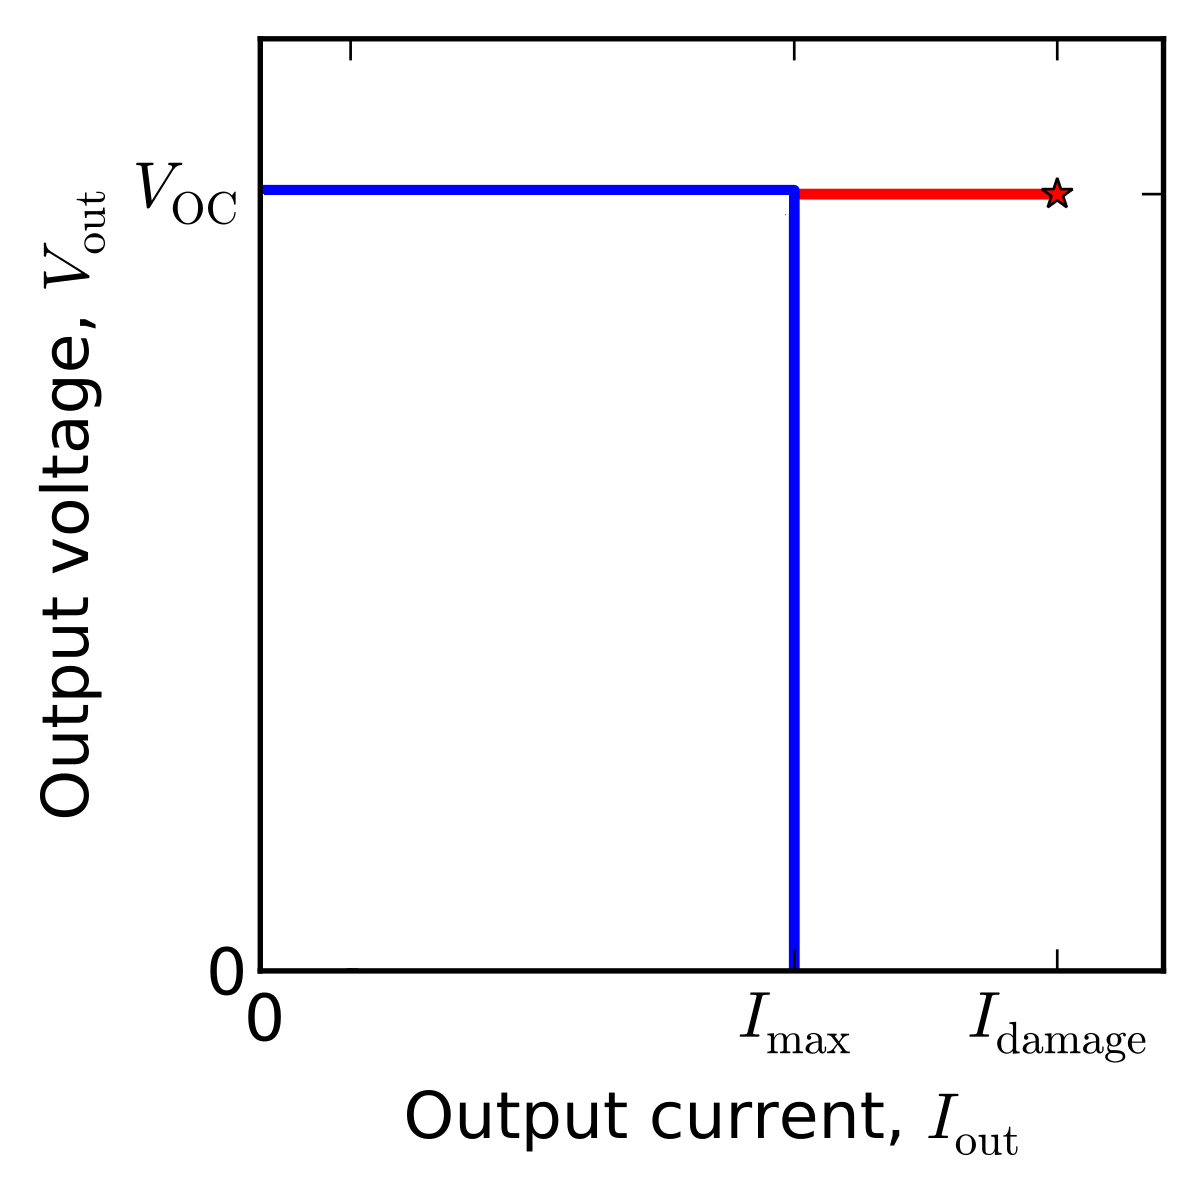
\includegraphics[width=0.5\textwidth]{ImagenesEjercicio2/Linearprotection.png}
	\caption{Característica de la Protección lineal.}
	\label{fig:circuitolinealcarac}
\end{figure}
Donde $I_{max}$ corresponde a la máxima corriente que uno define para el circuito e $I_{damage}$ es la corriente bajo la cual el circuito sufrirá un daño irreversible.\\
Se puede notar que en el  peor caso ($V_o = 0$) sería máxima tanto la corriente de salída como la caída de potencial sobre el transistor de paso, haciendo que por consecuente sea máxima la disipación de potencia sobre este, lo cual es un problema.
\subsubsection{Protección foldback}
La protección de Foldback es una variación de la lineal, la cual cuenta con 2 resistencias adicionales conectadas de la siguiente manera:
\begin{figure}[H]
\centering
	\includegraphics[width=0.5\textwidth, page=2]{ImagenesEjercicio2/Regulador.pdf}
	\caption{Circuito de Protección Foldback.}
	\label{fig:circuitofoldback}
\end{figure}
Si se desea resolver para $I_{o-Max}$ bastará con recorrer la malla:
\begin{align}
-I_{o-Max} \cdot R_a + V_{be} - (V_b-V_a)=0
\end{align}
\begin{align}
V_b=V_a \cdot \frac{R_c}{R_c+R_b}
\end{align}
\begin{align}
-I_{o-Max} \cdot R_a + V_{be} + V_a \cdot (1-\frac{R_c}{R_c+R_b})=0
\end{align}
\begin{align}
-I_{o-Max} \cdot R_a + V_{be} + (I_{o-Max} \cdot R_a +V_o) \cdot \frac{R_b}{R_c+R_b}=0
\end{align}
lo cual despejando para $I_{o-Max}$ queda:
\begin{align}
I_{o-Max}=  \frac{V_o \cdot R_b + V_{be}\cdot (R_b+R_c)}{R_a \cdot R_c}
\label{eq:Imaxfoldback}
\end{align}
De aquí se puede ver que la corriente caerá en función de la tensión de salida hasta establecerse en una corriente fija para la carga nula denominada $I_{sc}$ la tiene un valor de.
\begin{align}
I_{sc} = V_{be} \cdot \frac{R_b+R_c}{R_a \cdot R_c}
\label{eq:Isc}
\end{align}
Luego graficando la curva se obtiene:
\begin{figure}[H]
\centering
	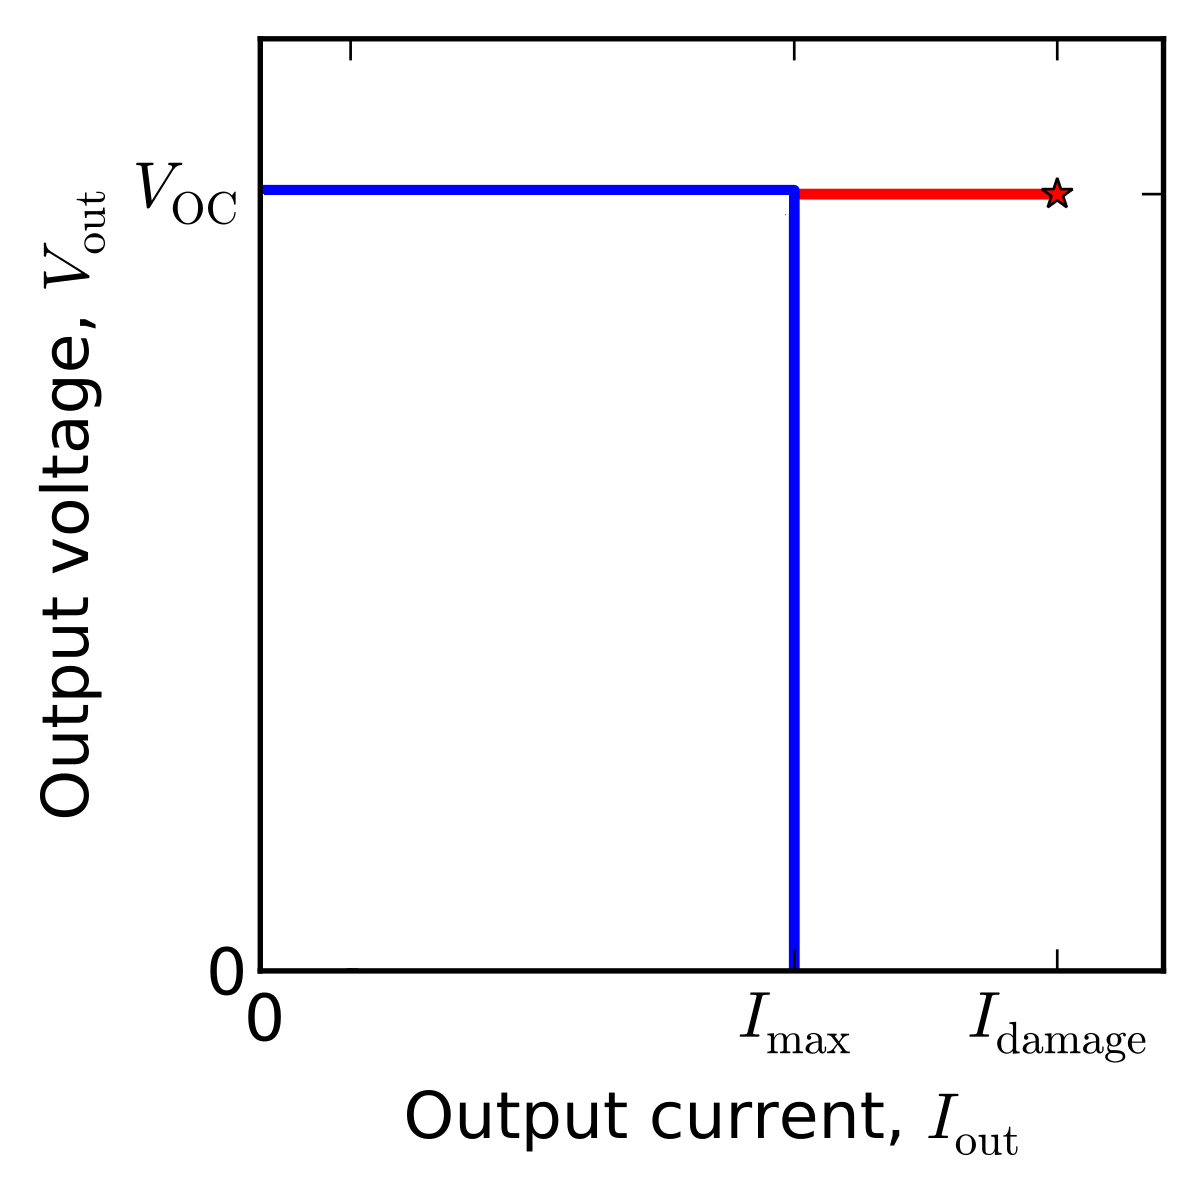
\includegraphics[width=0.5\textwidth]{ImagenesEjercicio2/foldbackLineal.png}
	\caption{Característica de la Protección foldback.}
	\label{fig:circuitofoldbackcarac}
\end{figure}
Se puede apreciar también la razón de su nombre dado que la curva de la corriente se ``dobla'' sobre si misma.\\
Si bien armar esta fuente resulta en una mayor cantidad de componentes, el hecho de que reduzca la corriente de paso al tener una carga nula, y que por ello reduzca la potencia consumida es un factor no menor. por esta razón esta fue la protección elegida a utilizar.\\
Solo a modo ilustrativo se grafica ambas curvas de las protecciones.
\begin{figure}[H]
\centering
	\includegraphics[width=0.5\textwidth]{ImagenesEjercicio2/foldback.png}
	\caption{Característica de la Protección foldback y lineal.}
	\label{fig:circuitofoldbacklinealcarac}
\end{figure}

%%%%%%%%%%%%%%%%%%%%%%%%%%%%%%%%%%%%%%%%%%%%%%%%%%%%%%%%%%%%%%%%%%%%%%
\subsection{Análisis de Componentes}
\subsubsection{Amplificador Operacional}
En la elección del amplificador operacional, se tuvieron en cuenta diversos componentes, como se ve a continuación en el siguiente cuadro comparativo:
\begin{table}[H]
\hspace*{-0.5cm}
\begin{tabular}{ccccccccc}
\hline
\textbf{Amplificador Operacional} & \textbf{GBP [Mhz]} & $\mathbf{SR [\frac{V}{\mu s}]}$ & $\mathbf{Z_{in} [\Omega]}$ & $\mathbf{Z_{out}[\Omega]}$ & $\mathbf{I_{bias}[A]}$ & $\mathbf{I_{off}[A]}$ & $\mathbf{V_{off}[mV]}$ & \textbf{THD} \\ \hline
\href{http://www.ti.com/lit/ds/symlink/tl082-n.pdf}{TL082}                   & 3                  & 13                              & 1T                         & -                          & 30p                 & 5p                    & 3                      & 0.003$\%$    \\
\href{http://www.ti.com/lit/ds/symlink/lm324-n.pdf}{LM324}                    & 1                  & 0.3                             & -                          & -                          & 45n                  & 5n                     & 2                      & -            \\
\href{http://www.ti.com/lit/ds/symlink/lm833.pdf}{LM833}                    & 10                 & 5                               & -                          & 37                         & 300n                & 10n                   & 0.3                    & 0.002$\%$    \\
\href{http://www.ti.com/lit/ds/symlink/lf356-mil.pdf}{LF356}                    & 2.5                & 12                              & 1T                         & -                          & 20p                 & 50p                   & 3                      & -            \\
\href{https://www.alldatasheet.com/datasheet-pdf/pdf/49039/AD/OP284.html}{OP284}                    & 4.25                & 4                              & -                         & 210 & 60n                 & 2n                   & 125m                      & $\leq 0.005\%$           \\
\href{http://www.ti.com/lit/ds/symlink/lm741.pdf}{LM741}                    & 1.5                & 0.5                             & 2M                         & 75                         & 80n                 & 20n                   & 2                      & -            \\
\href{http://www.ti.com/lit/ds/slos070d/slos070d.pdf}{NE5534}                   & 10                 & 13                              & 100k                       & 0.3                        & 500n                & 20n                   & 0.5                    & -           \\
\hline
\end{tabular}
\caption{Comparación de operacionales.}
\end{table}
También es notable que de todos los integrados el \textbf{OP284} es rail to rail, lo cual es de gran utilidad, si se desea obtener un valor de $V_1$ inferior, luego teniendo en cuenta el GBP, las corrientes de bias, la tension de offset, se optó por utilizar el OP284.
\subsubsection{Transistores de Paso}
Para la sección de transistor de paso, se eligió utilizar los transistores \href{https://pdf1.alldatasheet.com/datasheet-pdf/view/532914/FAIRCHILD/TIP31C.html}{QTIP41C} que son transistores de potencia, al igual que un \href{https://pdf1.alldatasheet.com/datasheet-pdf/view/2895/MOTOROLA/BC547C.html}{BC547C}, utilizando los TIP41C como el transistor que pasará la mayoría de la corriente y el BC547 como el que recibe la corriente del opamp.
Adicionalmente se le agrega una resistencia $R_5$ al emisor del BC547C con el objetivo de que en el analisis incremental el transistor se encuentren con un hfe estable.El valor de $R_5$ se obtiene a partir de la siguiente ecuación:
\begin{align}
\frac{V_{be}}{R_5}=I_{R5}\approx I_c
\end{align}
Para un valor de $13 \ mA$ corresponderá una resistencia de $56 \ \Omega$.
\subsubsection{Componentes de Protección}

Para la elección de estos componentes, se tuvo en cuenta la ecuación (\ref{eq:Imaxfoldback}) para la cual dado que se cuenta con dos grados de libertad se fijó $R_a$ a un valor fijo, así la potencia disipada en corto-circuito no es de un valor muy elevado, luego se fijó  $R_c$ lo cual definió inequivocamente $R_b$, también para el cálculo de estos valores se tuvo en cuenta que la máxima corriente ($2.5 \ A$) sería suministrada únicamente cuando se regule a la tensión máxima, y la pendiente de la curva de foldback fue seleccionada para que cuando baje la tensión de regulación aun tenga una corriente de salida máxima apreciable,teniendo en cuenta esto, quedan los valores
\begin{align}
R_a=0.56 \ \Omega  \ \ \ \ R_b=680 \ \Omega \ \ \ R_c=10 \ k\Omega \ \ \ I_{o-Max}=2.5 \ A \ \ \ I_{sc}= 1.34 \ A
\end{align}
Donde el valor de $I_{sc}$ queda fijo por la ecuación (\ref{eq:Isc}).

\subsubsection{Diodo de Referencia}
El diodo zener elegido fue el \href{https://d1d2qsbl8m0m72.cloudfront.net/en/products/databook/datasheet/discrete/diode/zener/bzx84b6v2lt116-e.pdf}{BZX84B6V2L}
debido a la estabilidad que cuenta para la $V_z$ y su reducida corriente de zener.\\
Es primordial que el diodo se encuentre bien polarizado para proveer una referencia estable, para ello se fijó una corriente de zener de $I_z =5.5 \ mA$, sabiendo que $V_z=6.2 \ V$  y utilizando la ecuación (\ref{eq:referencia}) se llega a un valor $R_Z=120 \ \Omega$ siendo adicionalmente el valor de $V_2$ definido en la sección (\ref{sec:fuentes}).
Luego el valor de $R_2$ será discutido en la sección (\ref{sec:resdet})
\subsubsection{Fuentes de Alimentación}
\label{sec:fuentes}
En la elección de la fuente de alimentación se buscó el $V_{1min}$ tal que el sistema regule, para esto simplemente se pidió que el transistor de paso no se encuentre saturado en regulación, en otras palabras:

\begin{align}
V_{1min}=V_{CEsat}+V_{Oreg}= 1.4 \ V+9 \ V=10.4 \ V
\end{align}
Otro punto de interés es la tensión a la salida del operacional, la cual no debe ser mayor a la de alimentación del mismo, para obtener la tensión en este nodo basta con seguir el ciruito y se verá que:
\begin{align}
V_{Out-opamp}= V_o+2\cdot V_{be} = 11.65V
\end{align}
Obteniendo que la máxima tensión de salida en el opamp coincide con el $V^+$.\\
Luego, dado que este es el mínimo absoluto, se dejará cierto margen de error, para la tensión de saturación del transistor, al igual que para variaciones en la tensión de linea, las cuales puedan saturar alguno de los transistores, por lo cual se eligió un valor de $V_1=14 \ V$.\\
Finalmente para $V_2$ se fijó un valor que sea levemente mayor a la $V_z$ del diodo elegido, tal que con el valor de resistencai $R_Z$ elegido se encuentre polarizado correctamente, por lo que se fijó $V_2=7\ V$.



\subsubsection{Resistencia circuito de detección}
\label{sec:resdet}
Dado que la salida en regulación depende directamente de la ecuación (\ref{eq:vovz}) basta con definir un valor de $R_1$ tal que $V_o=9 \ V$ dado que la $R_1$ será un potenciómetro con el cual se variará la tensión de regulación.\\ Así queda definido: $R_1= 10 \ k\Omega$ (potenciómetro) y $R_2=6.8  \  \Omega$
%%%%%%%%%%%%%%%%%%%%%%%%%%%%%%%%%%%%%%%%%%%%%%%%%%%%%%%%%%%%%%%%%%%%%%
\subsection{Análisis de cargas}
En la búsqueda de la carga mínima, basta con una vez definida la máxima corriente y la máxima tensión de regulación, queda:

\begin{equation}
	R_{Lmin} = \frac{V_{Omax}}{I_{Omax}} = 3.6 \ \Omega
\end{equation}
Luego la máxima carga corresponde a $R_l = \infty$
%%%%%%%%%%%%%%%%%%%%%%%%%%%%%%%%%%%%%%%%%%%%%%%%%%%%%%%%%%%%%%%%%%%%%%
\subsection{Análisis de Potencia}

\subsubsection{Amplificador Operacional}

\subsubsection{Transistores}

\begin{figure}[H]
\centering
	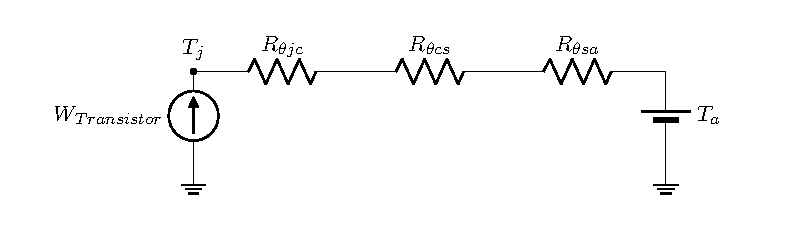
\includegraphics[width=0.6\textwidth, page=1]{ImagenesEjercicio2/Potencia.pdf}
	\caption{Circuito térmico para el cálculo de disipador del transistor.}
	\label{fig:circuitopottrans}
\end{figure}

\begin{equation}
\frac{T_j - T_a}{R_{\theta jc}+R_{\theta cs}+R_{\theta sa}} = P
\end{equation}

Asumiendo una temperatura ambiente de $40 \ \degree C$; una temperatura máxima de juntura en funcionamiento de $140 \ \degree C$, $20 \ \degree C$ menor a la especificada por el fabricante; la $R_{\theta jc}$ también especificada, de $3.125 \ \frac{\degree C}{W}$; el uso de una grasa siliconada de 0.002 pulgadas de espesor con una resistencia térmica de $204 \ \frac{\degree C \cdot inch}{W}$, y área estándar de un empaquetado de TO-220 de $0.41\cdot 0.59 \ inch^2$, obteniendo una $R_{\theta cs}$ de $1.6866 \frac{\degree C}{W}$; y finalmente una potencia disipada de $9.6 \ W$, levemente mayor a la máxima disipada; se obtiene

\begin{equation}
R_{\theta sa} = 4.57  \  \frac{\degree C}{W}
\end{equation}
\subsubsection{Diodos y Resistencias}

%%%%%%%%%%%%%%%%%%%%%%%%%%%%%%%%%%%%%%%%%%%%%%%%%%%%%%%%%%%%%%%%%%%%%%
\subsection{Simulaciones}
\subsubsection{Respuesta en régimen transitorio de Regulación}
La respuesta transitoria del sistema se asemeja a la de un sistema de segundo orden como se observa a continuación:\footnote{Todos los gráficos a continuación fueron realizados con una carga igual a la mínima que el sistema soporta}
\begin{figure}[H]
\centering
	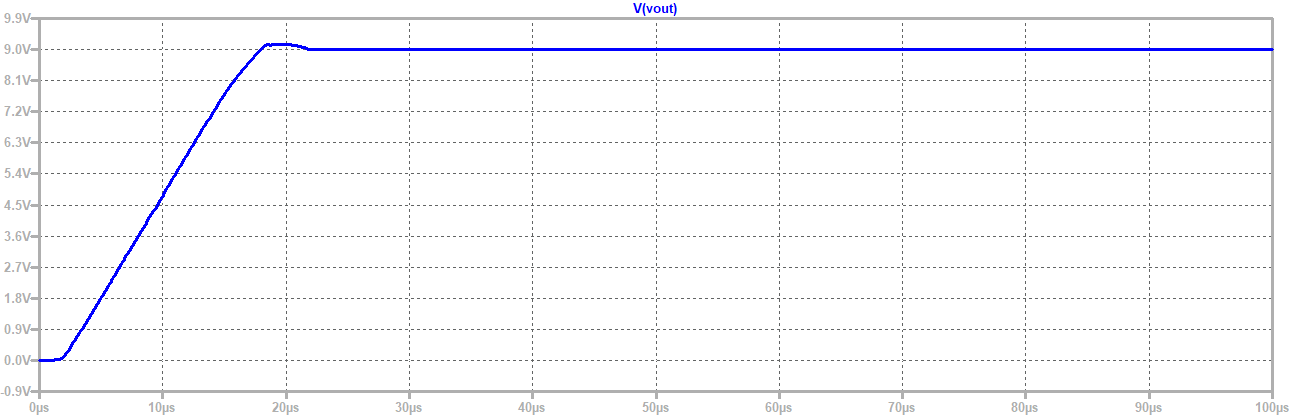
\includegraphics[width=1\textwidth]{ImagenesEjercicio2/transresp.png}
	\caption{Respuesta transitoria.}
	\label{fig:transitorioFuente}
\end{figure}
Es notable señalar, que el sobrepico del sistema alcanza 9.15V, lo cual es un 1.6$\%$ de desvío respecto de la tensión de regulación, y también observar que el tiempo de establecimiento del sistema es aproximadamente $22 \ \mu s$.\\
Además se simuló el circuito siendo afectado por ruido, con una frecuencia de 10kHz y una amplitud de 0.5V, estos valores fueron elegidos asi es apreciable la variación  durante el transitorio.
\begin{figure}[H]
\centering
	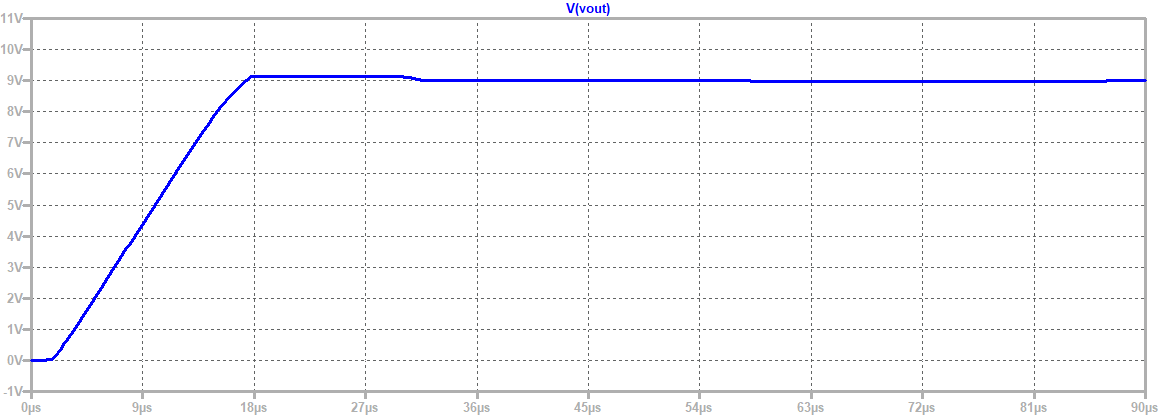
\includegraphics[width=1\textwidth]{ImagenesEjercicio2/transrespnoise.png}
	\caption{Respuesta transitoria con ruido.}
	\label{fig:transitorioFuentenoise}
\end{figure}
Si bien la imagen es realmente similar, esto se debe a la frecuencia del ruido, aun así se puede apreciar una diferencia de las pequeñas oscilaciones generedadas por el ruido en la tensión estabilizada en 9V. En cuanto a los parámetros del transitorio, el máximo sobrepico alcanzado es de 9.15V y el tiempo de establecimiento es de aproximadamente $32 \ \mu s$.
\subsubsection{Respuesta en régimen permanente de Regulación}
En el caso del regiment permantente se verá la capacidad de mantener al tensión regulada en la salida.
En el caso de que la señal no tenga ruido la tensión regulada será $9 \ V$ sin ningún tipo de variación.
\begin{figure}[H]
\centering
	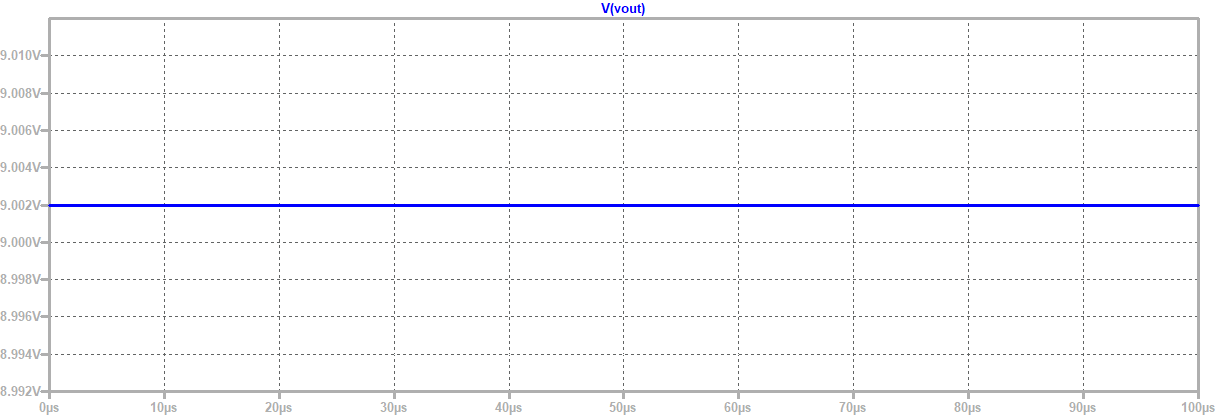
\includegraphics[width=1\textwidth]{ImagenesEjercicio2/permresp.png}
	\caption{Respuesta en régimen permanente.}
	\label{fig:permanenteFuente}
\end{figure}
Lo cual es perfectamente esperable, ahora veremos como es la respuesta frente a señales con distintos tipos de contaminación.
Para la primer prueba se vera la señal original, con la adición de una señal senoidal de $10 \ kHz$ de amplitud $0.5 \ V$.
La salida es la siguiente:
\begin{figure}[H]
\centering
	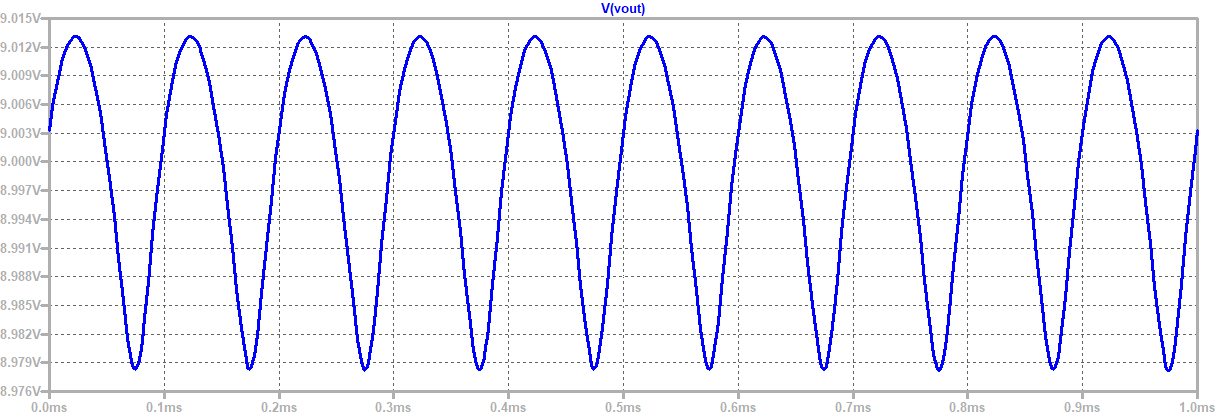
\includegraphics[width=1\textwidth]{ImagenesEjercicio2/permrespsine.png}
	\caption{Respuesta en régimen permanente con ruido senoidal.}
	\label{fig:permanenteFuentesine}
\end{figure}
Se puede ver que el desvío respecto de los $9 \ V$ es del $0.14\%$.
Luego se agregó adicionalmente una señal triangular de frecuencia $50 \ Hz$ y amplitud unitaria.
\begin{figure}[H]
\centering
	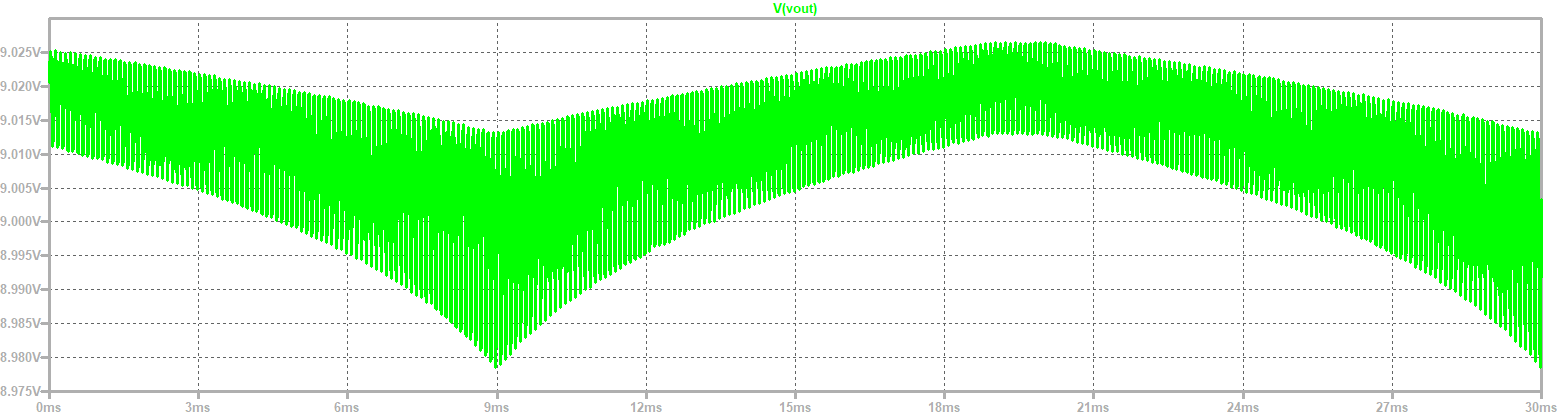
\includegraphics[width=1\textwidth]{ImagenesEjercicio2/permrespsinetri.png}
	\caption{Respuesta en régimen permanente con ruido senoidal y triangular.}
	\label{fig:permanenteFuentesinetri}
\end{figure}
Es notable que incluso con estas dos fuentes de ruido, de distinta amplitud y frecuencia el sistema continúa regulando con un desvio no mayor del $0.24\%$.
\subsubsection{Respuesta en Frecuencia}
\subsubsection{Curva de Foldback}
La curva correspondiente al foldback fue simulada y graficada como se ve a continuación:
\begin{figure}[H]
\centering
	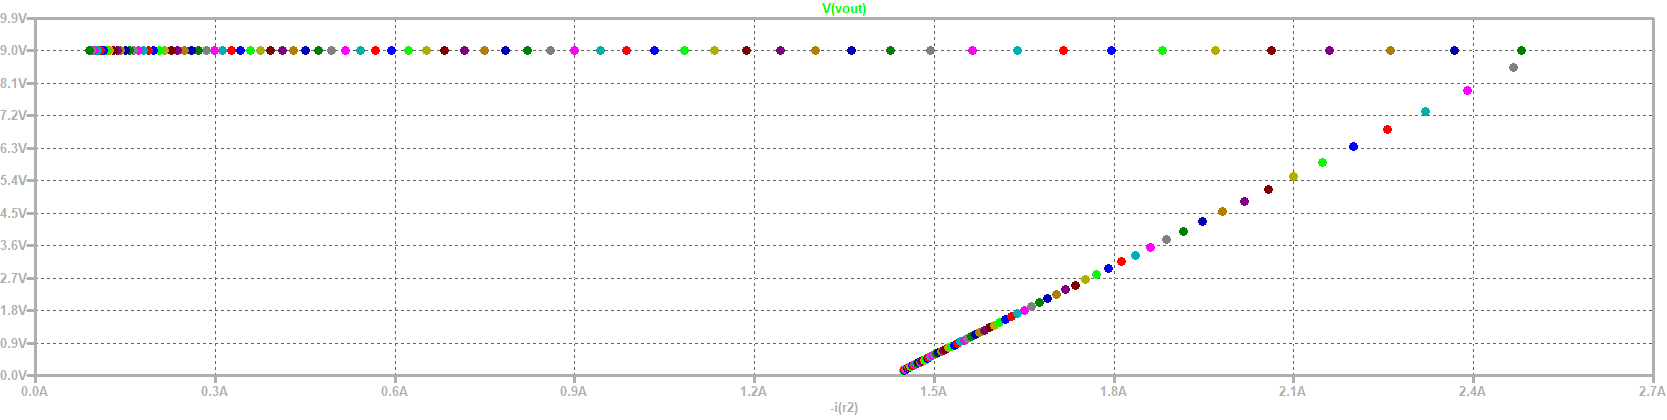
\includegraphics[width=1\textwidth]{ImagenesEjercicio2/curvefoldback.png}
	\caption{Curva de Foldback.}
	\label{fig:GraficoFOldbacki}
\end{figure}
Se puede apreciar, que la máxima corriente es de 2.5A como fue calculado al igual que el valor de $I_{sc}$, vale la pena mencionar que a medida que se varíe la $R_1$ variará la corriente máxima de salida acorde a la ecuación (\ref{eq:Imaxfoldback})
\subsubsection{Impedancia de Salida}
La impedancia de salida fue simulada y graficada:
\begin{figure}[H]
\centering
	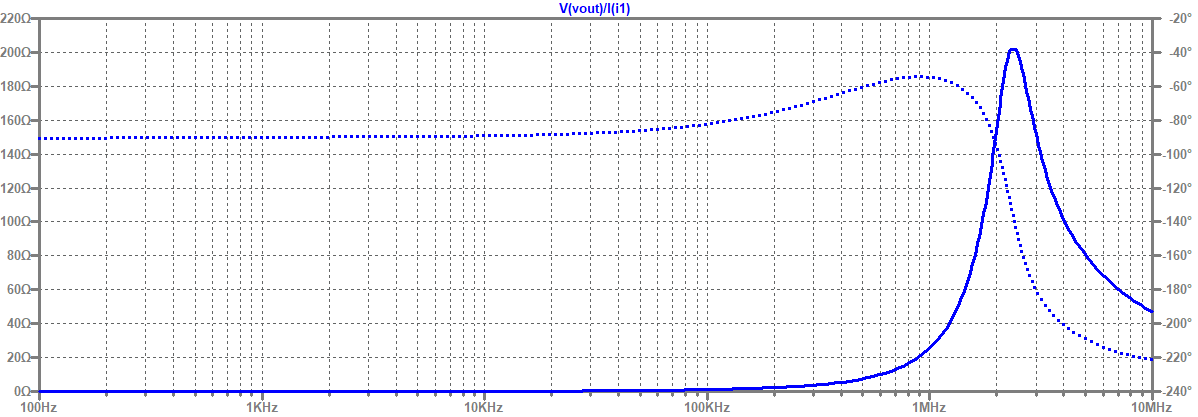
\includegraphics[width=1\textwidth]{ImagenesEjercicio2/zoutspice.png}
	\caption{Impedancia de salida.}
	\label{fig:zout}
\end{figure}
Se observa que la impedancia de salida es baja para la mayor parte del espectro, no superando nunca los 220$\Omega$.
\subsubsection{Potencias}
En esta sección se simularon las curvas de potencias sobre los componentes al variar la carga del circuito.\\
\begin{itemize}
\item Diodo Zener: 
Se puede ve que la máxima potencia disipada corresponde a la mínima caraga, dicha potencia es de 37mW lo cual no es un problema para dicho diodo.
\begin{figure}[H]
\centering
	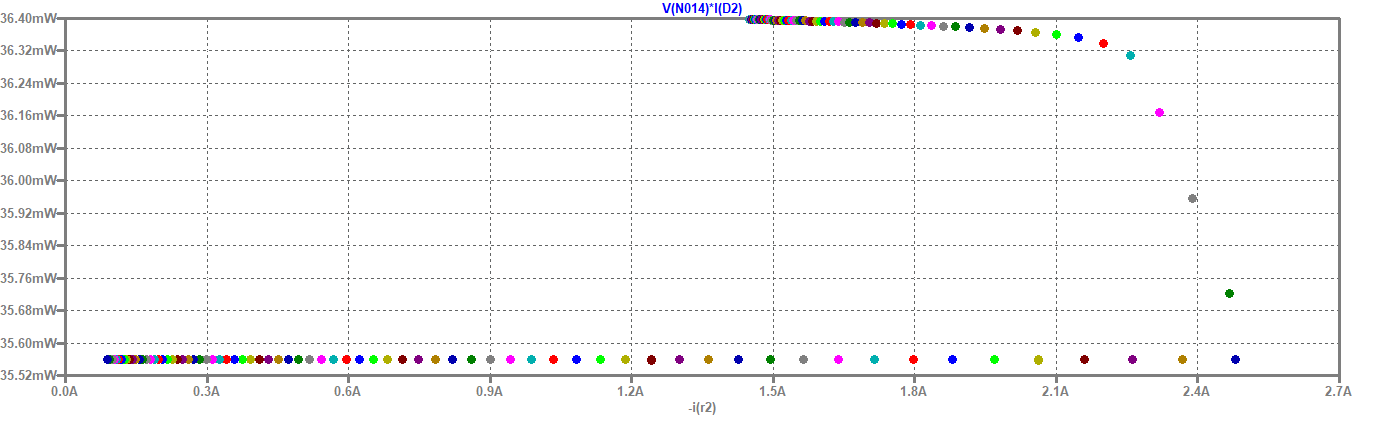
\includegraphics[width=1\textwidth]{ImagenesEjercicio2/potzener.png}
	\caption{Potencia sobre el zener.}
	\label{fig:potzener}
\end{figure}
\item BC547C Darlington: La máxima potencia es de 330mW lo cual no es un problema para dicho transistor, al igual que la anterior curva se observa un aumento considerable una vez que se activa el foldback, pero aun en la zona de operación tiene una pendiente.
\begin{figure}[H]
\centering
	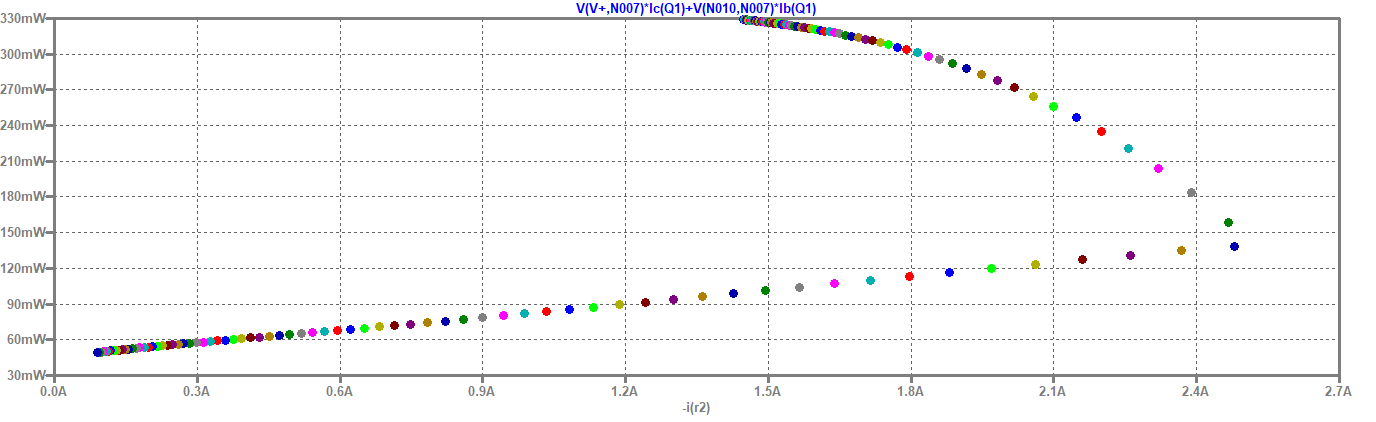
\includegraphics[width=1\textwidth]{ImagenesEjercicio2/potbc547.png}
	\caption{Potencia sobre el BC547C del darlington.}
	\label{fig:potbc547}
\end{figure}
\item $R_a$: La potencia máxima disipada corresponde a 3.5W lo cual es esperado dado que es $R_a\cdot I_{max}^2$ 
\begin{figure}[H]
\centering
	\includegraphics[width=1\textwidth]{ImagenesEjercicio2/potra.png}
	\caption{Potencia sobre la $R_a$.}
	\label{fig:potra}
\end{figure}
\item TIP31C: La potencia sobre estos transistores de potencia es de 9W, lo cual indica que un disipador debe ser utilizado para su correcto funcionamiento.
\begin{figure}[H]
\centering
	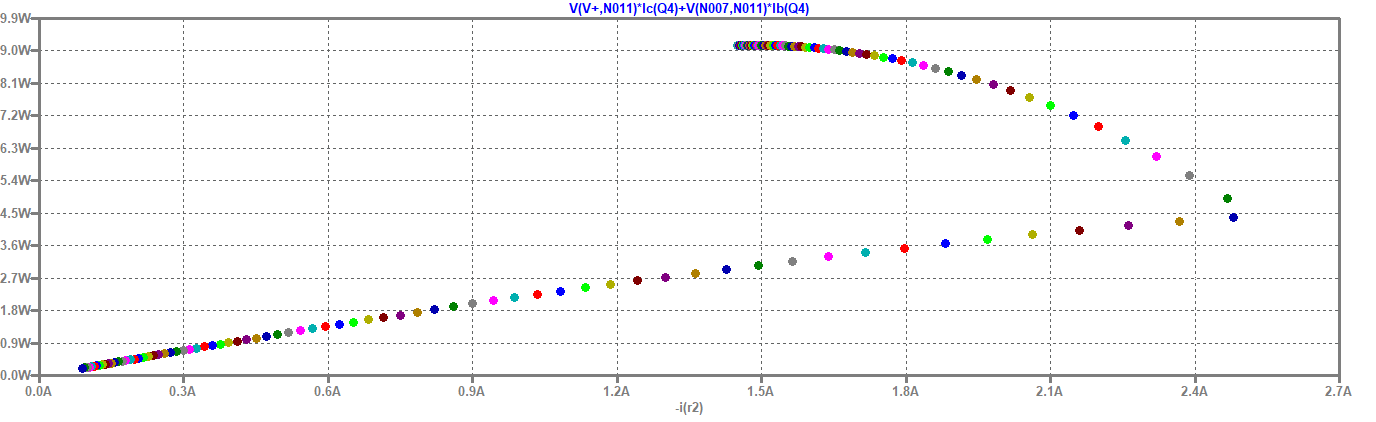
\includegraphics[width=1\textwidth]{ImagenesEjercicio2/pottip31c.png}
	\caption{Potencia sobre el TIP31C.}
	\label{fig:pottip31}
\end{figure}
\item BC547 Protección: Se debe notar que el transistor consume nada de potencia, hasta el momento en el cual se activa, alcanzando un limite de 60mW.
\begin{figure}[H]
\centering
	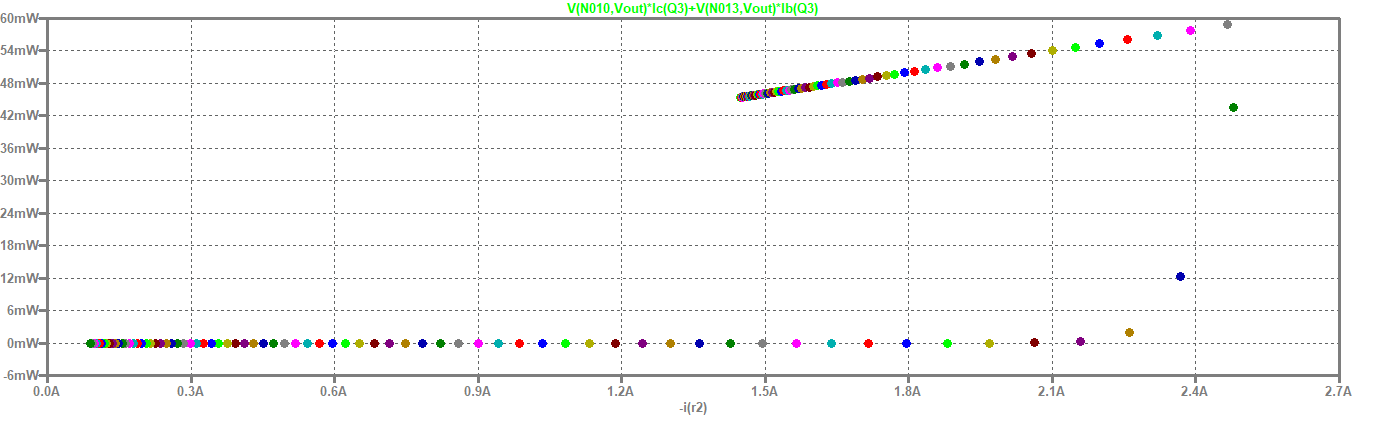
\includegraphics[width=1\textwidth]{ImagenesEjercicio2/potprot.png}
	\caption{Potencia sobre el BC547C de la protección.}
	\label{fig:potbc547prot}
\end{figure}
\item Operacional: Para el operacional se observa que la máxima potencia corresponde a 330mW para la carga nula, y vale la pena mencionar que al medir la potencia en spice, tambien son consideradas las corrientes de alimentación.
\begin{figure}[H]
\centering
	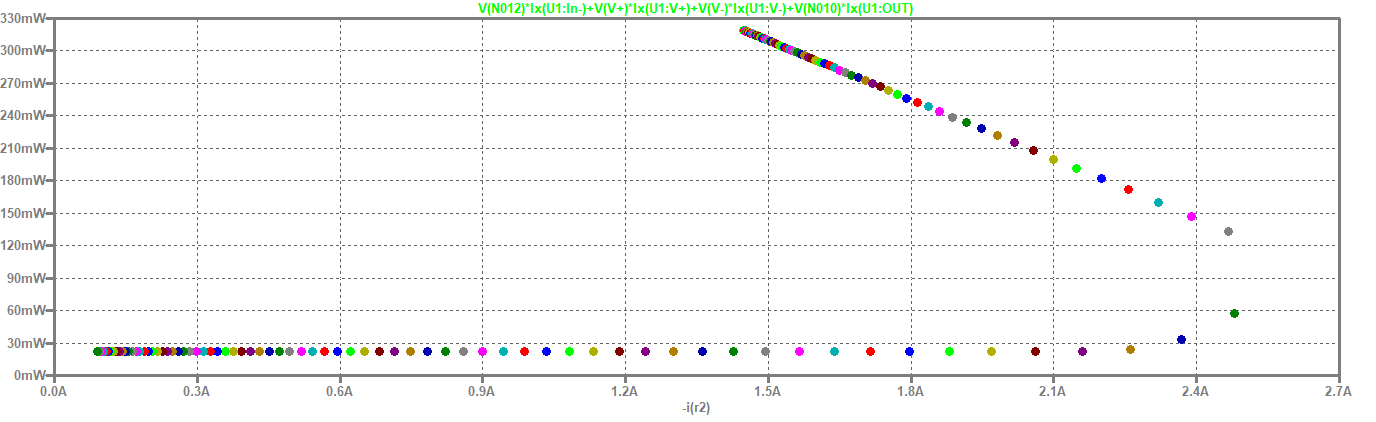
\includegraphics[width=1\textwidth]{ImagenesEjercicio2/potopamp.png}
	\caption{Potencia sobre el operacional.}
	\label{fig:potop}
\end{figure}
\item Carga: Se observa que el crecimiento es lineal hasta la activación de la protección y luego sigue la curva del foldback, teniendo una potencia máxima de 22.5W.
\begin{figure}[H]
\centering
	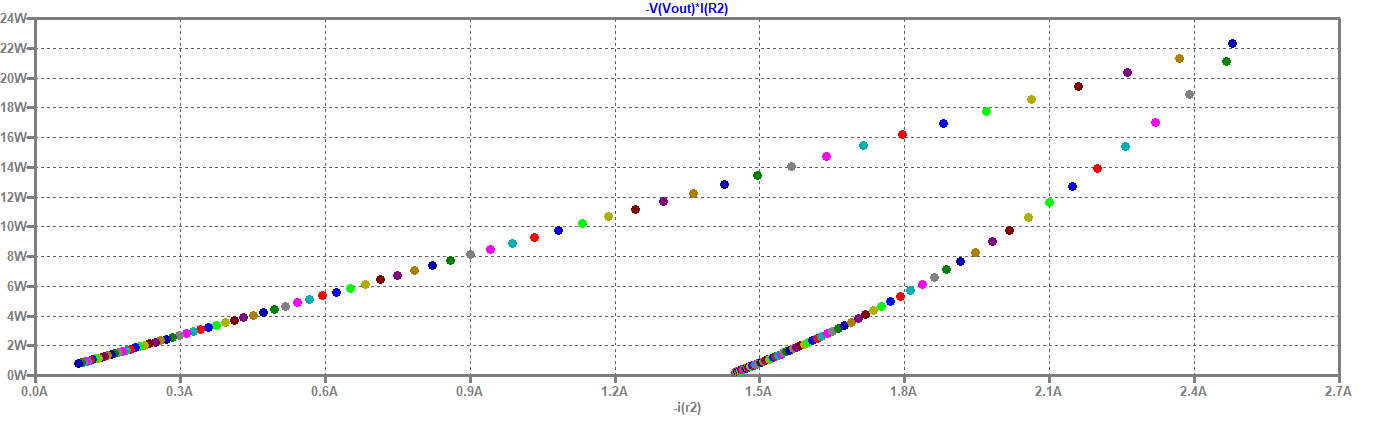
\includegraphics[width=1\textwidth]{ImagenesEjercicio2/potload.png}
	\caption{Potencia sobre la carga.}
	\label{fig:potload}
\end{figure}
\end{itemize}




%%%%%%%%%%%%%%%%%%%%%%%%%%%%%%%%%%%%%%%%%%%%%%%%%%%%%%%%%%%%%%%%%%%%%%
\subsection{Conclusiones}











En la siguiente sección, se busca elaborar una fuente regulada de tensión que cumpla con una salida que varíe entre $0 \ V$ y $9 \ V$, con una corriente de salida máxima de $2.5 \ A$. Dado que la tensión mínima debe ser nula, se implementó un regulador serie que utiliza un lazo de realimentación negativa que muestrea tensión y suma corriente, siendo así el circuito resultante el presentado a continuación.
%\begin{figure}[H]
%\centering
%	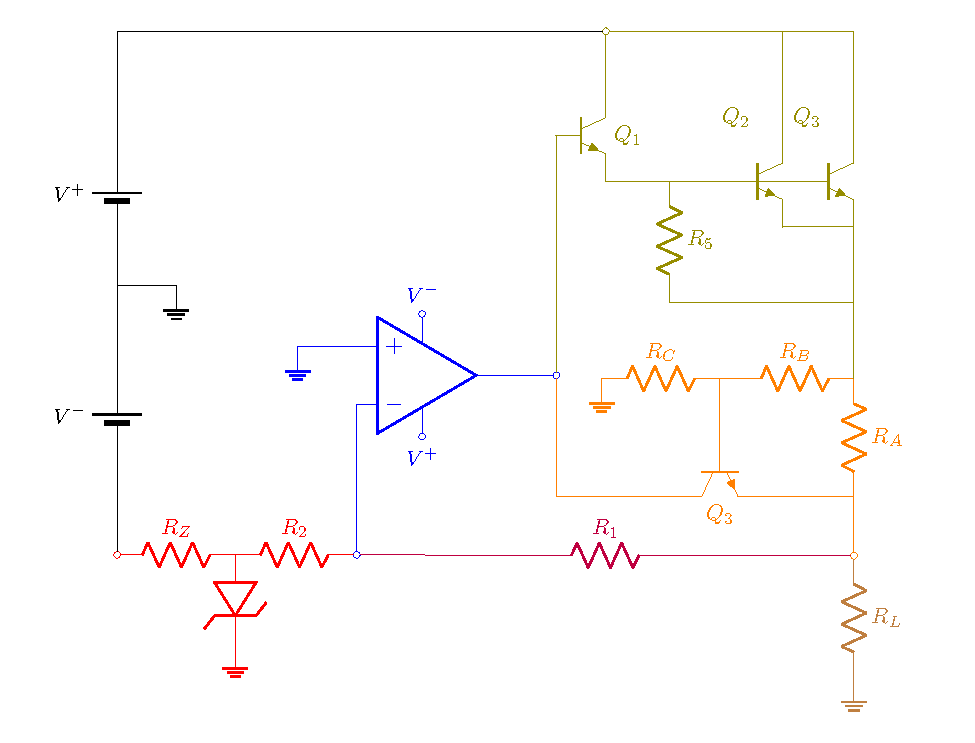
\includegraphics[width=0.8\textwidth, page=1]{ImagenesEjercicio2/Regulador.pdf}
%	\caption{Circuito regulador de tensión.}
%	\label{fig:circuito1}
%\end{figure}
%
%En la Figura (\ref{fig:circuito1}) se puede observar en distintos colores las diferentes etapas del sistema, siendo \textcolor{blue}{en azul el amplificador error}, \textcolor{olive}{en verde el transistor de paso}, \textcolor{red}{en rojo el elemento de referencia}, \textcolor{purple}{en violeta el circuito de detección} y \textcolor{orange}{en naranja el circuito de protección}.

\begin{equation}
\frac{V^- - V_Z}{R_Z} + I_Z = \frac{V_Z}{R_9}
\end{equation}






El pre-regulador cumple la función de brindar corriente \textbf{(habría que desarrollar un poco más)}. Para el caso presente, se observa que el amplificador operacional puede llegar hasta temperaturas de $125 \ ^o C$ son problema. Asumiendo una temperatura ambiente de $40 \ ^o C$, la potencia máxima disipada por operacional es de $0.7 \ W$.
\begin{figure}[H]
\centering
	\includegraphics[width=0.6\textwidth, page=2]{ImagenesEjercicio2/Potencia.pdf}
	\caption{Circuito equivalente de potencias con $R_{\theta a-j} = 103 \ \frac{^o C}{W}$.}
	\label{fig:circuitopot}
\end{figure}

Es por ello que se analiza la potencia tanto en regulación como fuera de esta. Durante la primer etapa, la tensión de salida $V_O$ es estable pero la corriente es cada vez mayor. A pesar de esto, la potencia disipada por el opamp se mantiene menor a la máxima. Por otro lado, con el circuito fodlback activado, la tensión decae, haciendo que también decaiga la potencia del amplificador, manteniendola por debajo del máximo.
\begin{figure}[H]
\centering
	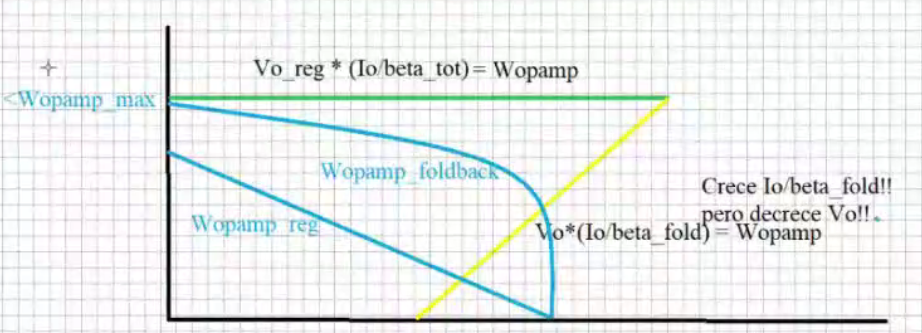
\includegraphics[width=0.6\textwidth]{ImagenesEjercicio2/Potencia2.png}
	\caption{Curvas de potencia consumida.}
	\label{fig:curvapot}
\end{figure}


\end{document}